\documentclass[12pt,fleqn]{article}

\usepackage[utf8]{inputenc}
\usepackage[T2A]{fontenc}
\usepackage{amssymb,amsmath,mathrsfs,amsthm}
\usepackage[russian]{babel}
\usepackage[pdftex]{graphicx}
\usepackage{multirow}
\usepackage[footnotesize]{caption2}
\usepackage{indentfirst}
\usepackage[colorlinks,linkcolor=black,citecolor=black, unicode]{hyperref}

\usepackage{xcolor}
\usepackage{sectsty}
\usepackage{pgfplots}
%\usepackage{wrapfig}


% Параметры страницы
\textheight=24cm % высота текста
\textwidth=16cm % ширина текста
\oddsidemargin=0pt % отступ от левого края
\topmargin=-2.5cm % отступ от верхнего края
\parindent=24pt % абзацный отступ
\parskip=0pt % интервал между абзацам
\tolerance=2000 % терпимость к "жидким" строкам
\flushbottom % выравнивание высоты страниц

\renewcommand{\baselinestretch}{1.1}

%math operatons
\newcommand{\norm}{\mathop{\rm norm}\limits}
\newcommand{\real}{\mathbb{R}}
\newcommand{\ex}{\mathbb{E}}
\newcommand{\diag}{\mathrm{diag}}
\newcommand{\intset}{\mathrm{int}}
\newcommand{\softmax}{\mathop{\rm softmax}\limits}
\newcommand{\lossfunc}{\mathcal{L}'}
\newcommand{\elbo}{\mathcal{L}}
\newcommand{\normal}[3]{\mathcal{N}(#1 | #2, #3)}
\newcommand{\dd}[2]{\frac{\partial#1}{\partial#2}}
\newcommand{\kl}[2]{\mathop{KL}(#1 \parallel #2)}
\newcommand{\nm}{\mathcal{N}}
\newcommand{\sle}{\; \Rightarrow \;}
\newcommand{\indpos}{\mathbf{I}_{d_k}^{+}[i, j]}
\newcommand{\indneg}{\mathbf{I}_{d_k}^{-}[i, j]}



%my settings
\usepackage{titlesec}
\graphicspath{{../figures/}}
\titleformat*{\subsubsection}{\large\bfseries}


\begin{document}

\begin{titlepage}
    \begin{center}
        Московский государственный университет имени М. В. Ломоносова
    
        \bigskip
        
\includegraphics[width=50mm]{msu.pdf}
    
        \bigskip
        Факультет Вычислительной Математики и Кибернетики\\
        Кафедра Математических Методов Прогнозирования\\[10mm]
    
        \textsf{\large\bfseries
            КУРСОВАЯ РАБОТА СТУДЕНТА 317 ГРУППЫ\\[10mm]
            ''Математические и технологические проблемы
            построения графика в параллельных осях''
            \\[5mm]
            \textit{''Mathematical and technological problems of plotting parallel axes''}
        }\\[10mm]
        
    
        \begin{flushright}
            \parbox{0.5\textwidth}{
                Выполнил:\\
                студент 3 курса 317 группы\\
                \emph{Тыцкий Владислав Игоревич}\\[5mm]
                Научный руководитель:\\
                к.ф-м.н., доцент\\
                \emph{Майсурадзе Арчил Ивериевич}
            }
        \end{flushright}
    
        \vspace{\fill}
        Москва, 2021
    \end{center}
    \end{titlepage}

\newpage
\renewcommand{\contentsname}{Содержание}

\section*{Аннотация}
В анализе данных важной частью любого исследования является представление данных в наглядной для человека форме. 
Это необходимо не только для самого исследователя, но и для тех, кто читает исследование.
Для представления данных низкой размерности существует множество
вариантов визуализации. Однако далеко не все эти методы подходят для
высокоразмерных данных. В данной курсовой работе изучается диаграмма для визуализации
многомерных данных под названием ''график в параллельных осях'', рассмотрены его
многочисленные модификации, введены новые методы увеличения читаемости, а также 
представлен обзор собственной библиотеки визуализации данного графика.

\newpage

\tableofcontents

\newpage

\section{Введение}
В анализе данных важной частью любого исследования является представление данных\footnote{
Часто будут использоваться синонимы: выборка, датасет}
в наглядной для человека форме. 
Это необходимо не только для самого исследователя, но и для тех, кто читает исследование.

Для представления данных низкой размерности (до 3-ей) существует множество
вариантов визуализации. Однако далеко не все эти методы подходят для
высокоразмерных данных. Это является фундаментальной проблемой
представления информации на экране компьютера.
Её обходят по-разному: через представление координат (одной и более) как параметры и рисование нескольких
диаграмм для низкоразмерных данных, через рисование проекций на подпространства или через агрегирование
выборки. Но среди всех способов визуализации можно выделить так называемый график в
параллельных осях (parallel coordinates).

\begin{figure}[htb]
    \centering
    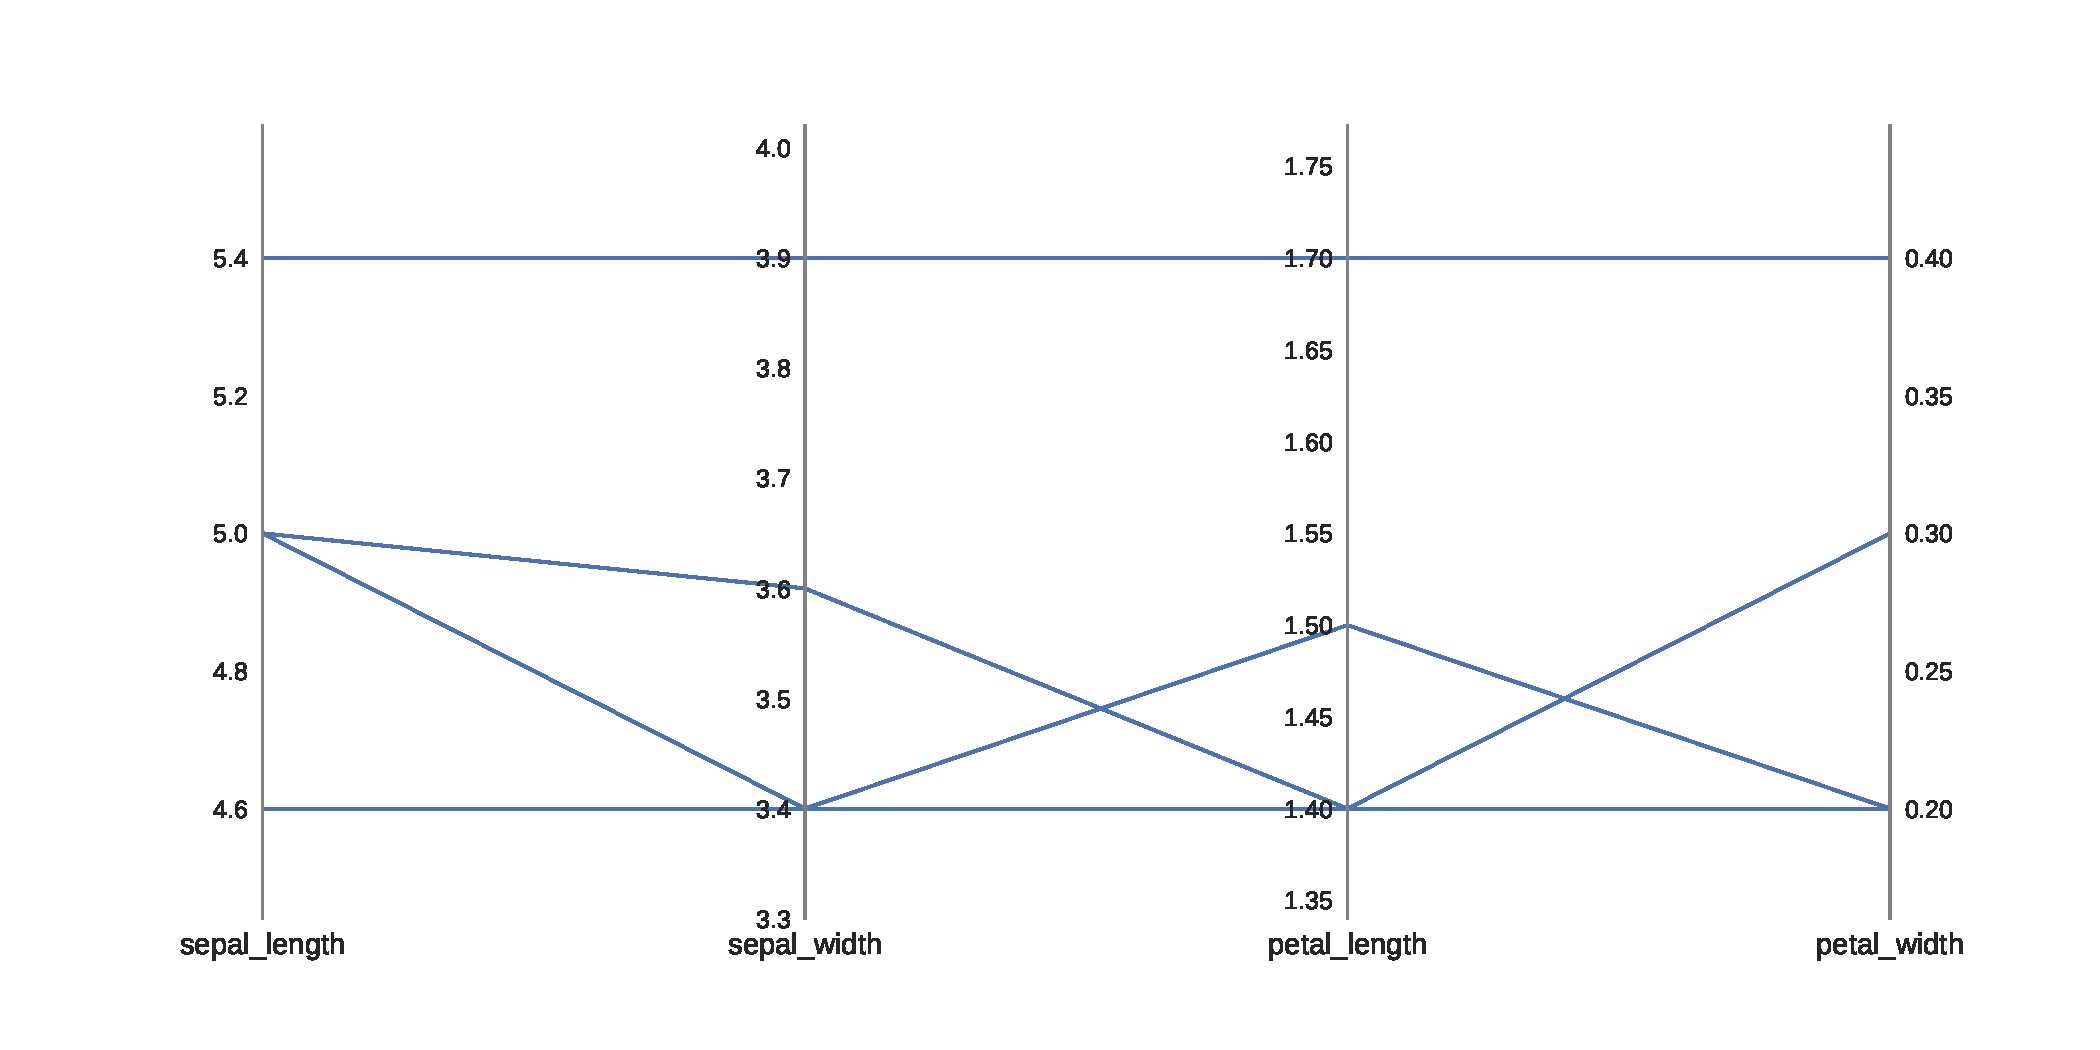
\includegraphics[width=15cm]{classic_pc.pdf}
    \caption{Классический график в параллельных осях}
    \label{classic_pc}
\end{figure}

График в параллельных осях --- метод визуализации многомерных данных.
Для отображения векторов в n-мерном пространстве рисуется n параллельных линий (осей) на одинаковом
расстоянии друг от друга. У каждой оси есть направление, а также положение относительно других осей. 
Вектор в пространстве представляется в виде ломаной кривой, с вершинами на параллельных осях. Точка пересечения
кривой с i-ой осью соответствует i-ой координате объекта. График позволяет ''увидеть'' не только поведение каждого
отдельного объекта, но и зависимости между соседними осями.\cite{inselberg_1985}

На данный момент исследователи редко используют график в параллельных осях в своих работах. Такое положение дел может 
быть связано с недостаточной читаемостью классических представлений графика, а также с практически полным отсутствием программных реализаций данного 
графика. 

\section{Модификации}

\subsection{Добавление меток}

Обычно классический график в параллельных осях используют в модифицированном виде ---
каждому объекту из выборки ставят в соответствие некоторую категориальную метку по какому-то правилу\footnote{
Правило выбирают так, чтобы объекты с одной меткой были ''похожими'' в некотором смысле. Иногда правило может естественным образом вытекать из самих данных,
например, различные виды растений. },
а далее линия, соответствующая объекту, окрашивается в некоторый цвет однозначный метке объекта.
Таким образом на графике можно проследить как ведут себя ''похожие'' объекты. 

\begin{figure}[htb]
    \centering
    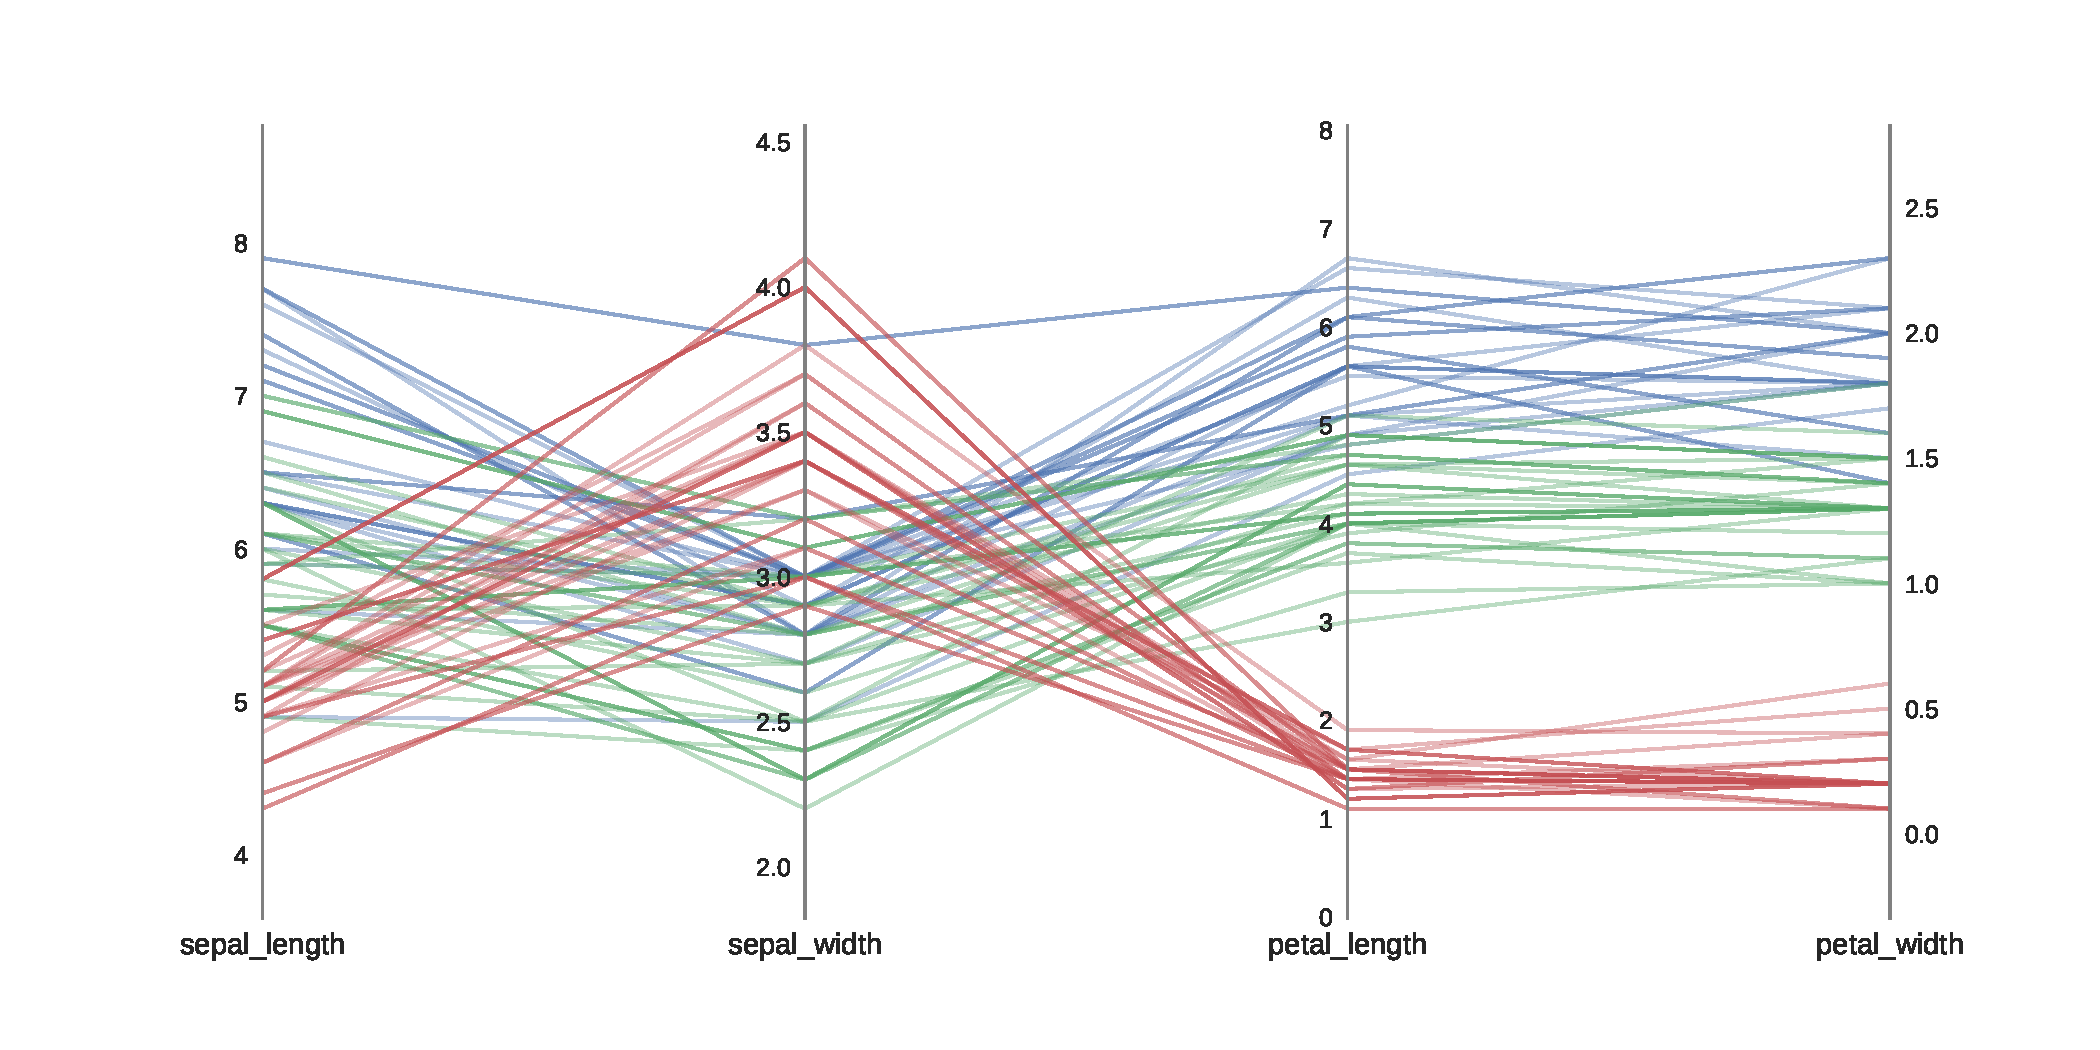
\includegraphics[width=15cm]{color_pc.pdf}
    \caption{График в параллельных осях с кластерами}
    \label{color_pc}
\end{figure}

На Рис. \ref{color_pc} можно наблюдать некоторые монотонные зависимости между признаками (осями) в рамках кластеров.


\subsection{Гладкие линии}

\begin{figure}[htb]
    \centering
    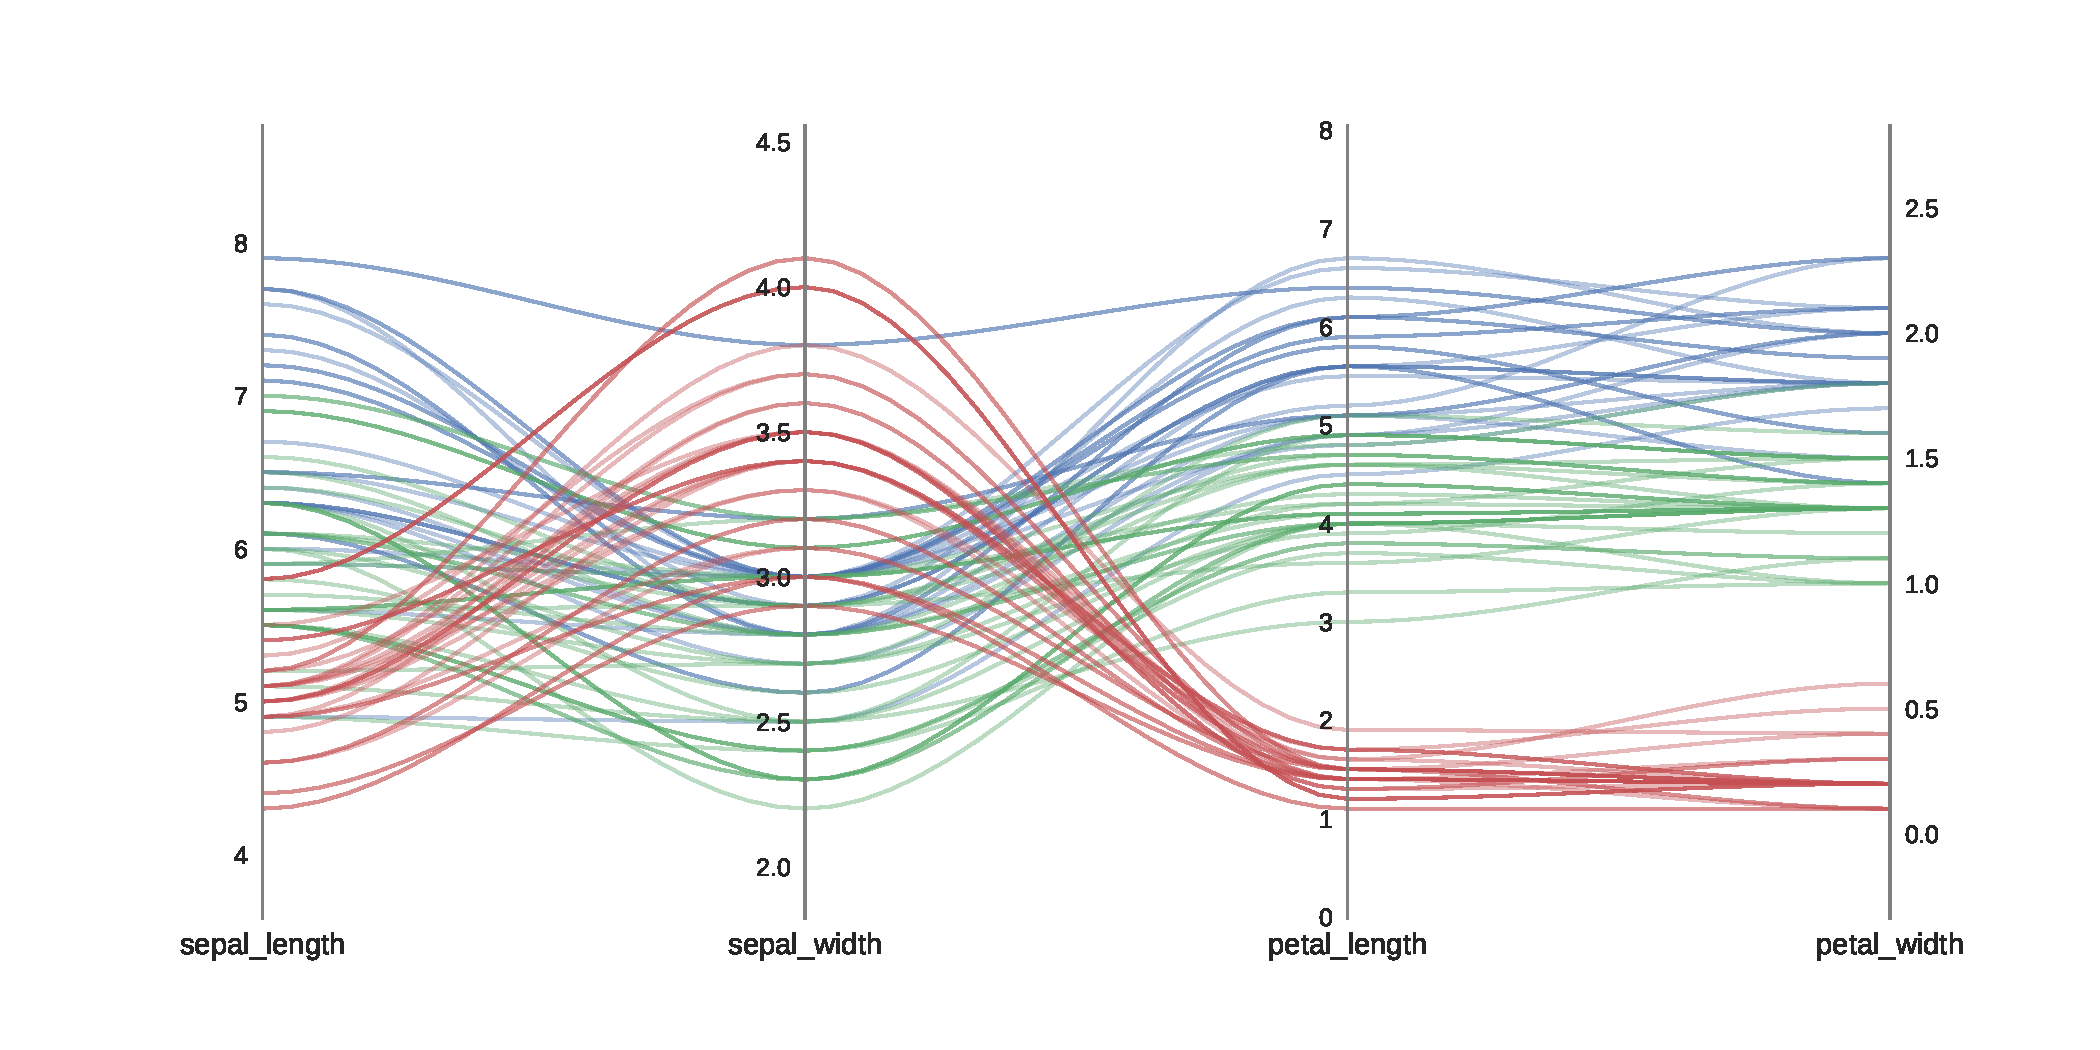
\includegraphics[width=15cm]{smooth_pc.pdf}
    \caption{График в параллельных осях с гладкими линиями}
    \label{smooth_pc}
\end{figure}

Нет никакой необходимости рисовать именно ломанные линии, можно рисовать гладкие кривые, 
которые ''входят'' под некоторым углом к оси (чаще всего перпендикулярно).
Человеку легче воспринимать гладкие линии, поэтому
читаемость графика может возрасти.\cite{state_of_the_art}

\newpage

\subsection{Связывание линий}

\begin{figure}[htb]
    \centering
    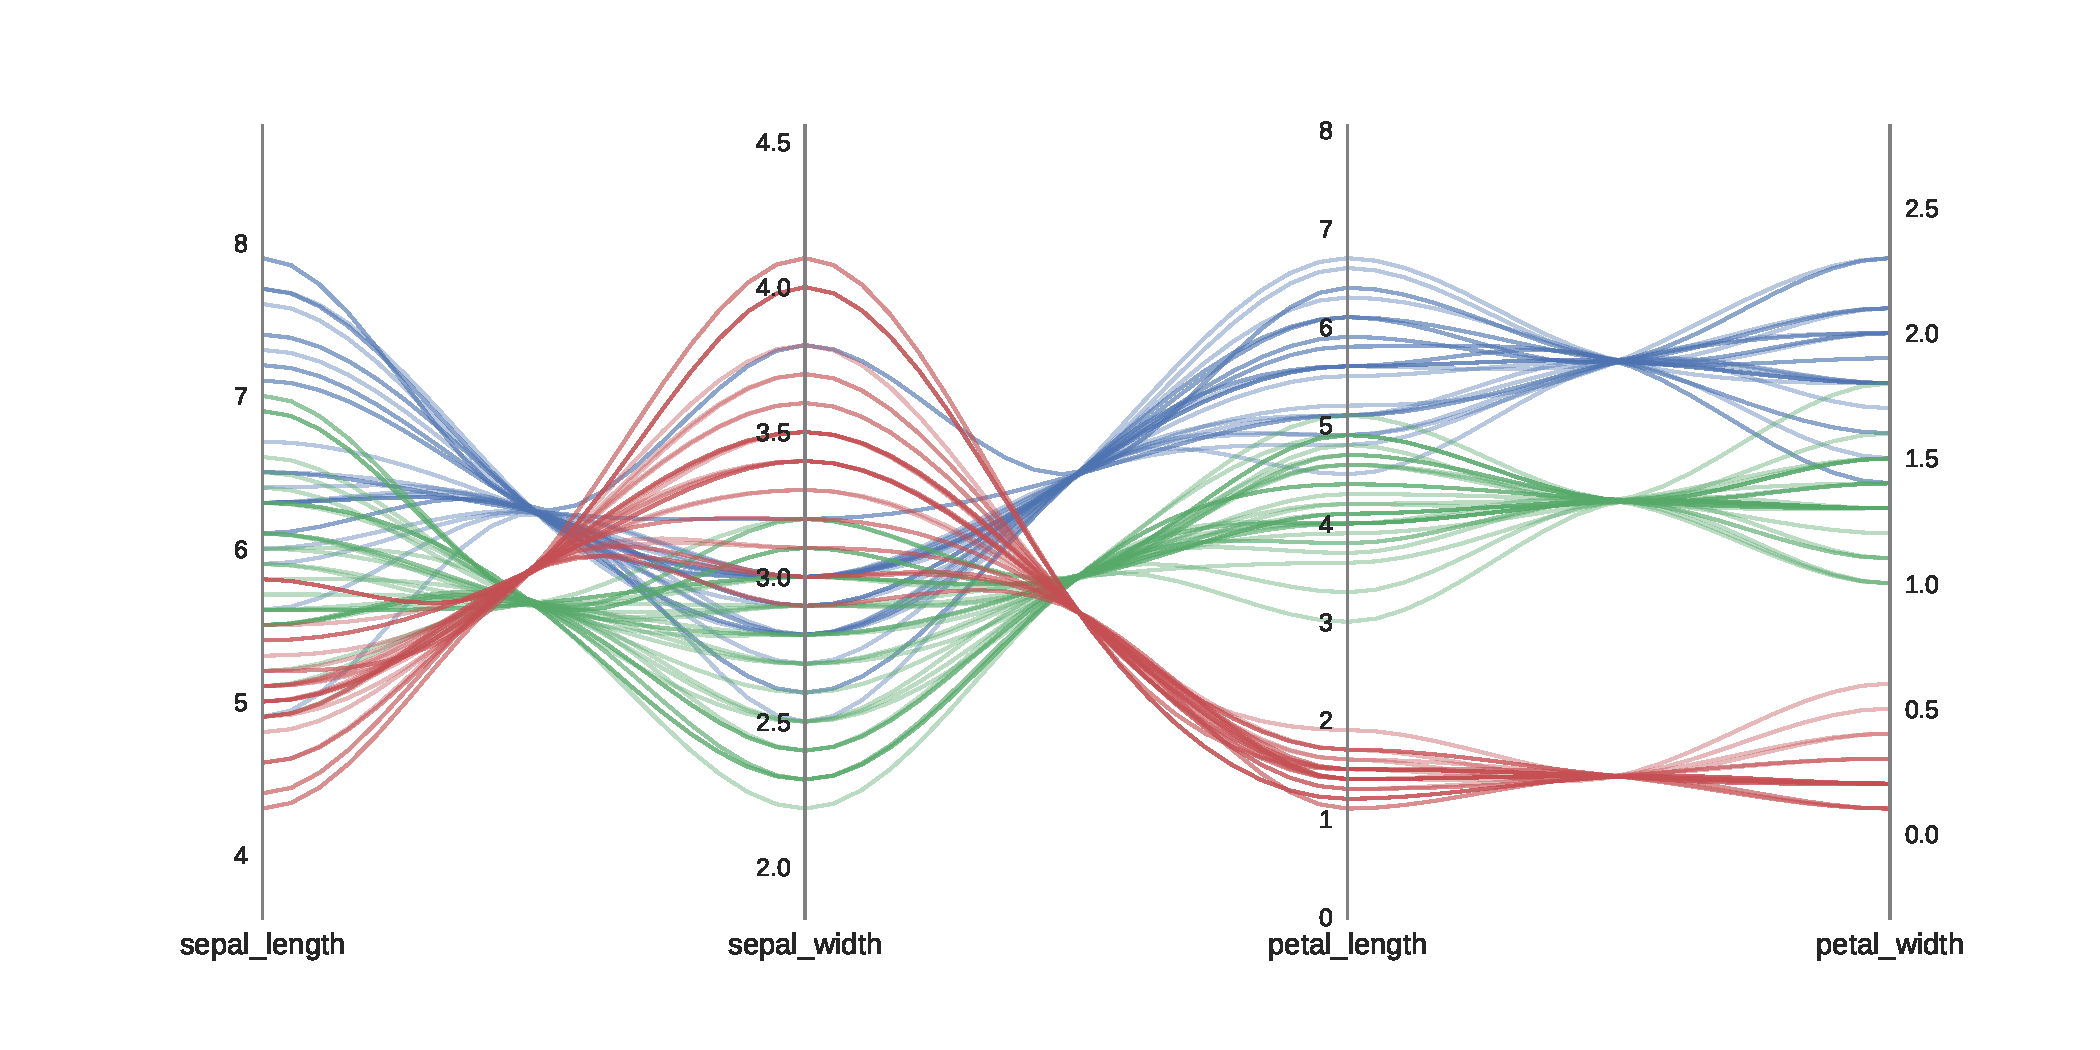
\includegraphics[width=15cm]{bundle_0.01_pc.pdf}
    \caption{График в параллельных осях со ''жгутами''}
    \label{bundle0.01_pc}
\end{figure}

Линии с одинаковыми метками могут связываться в ''жгут'' между парой осей, а 
далее распадаться к соответствующим точкам на оси. Степень связанности регулируема. В таких графиках
теряется читаемость в рамках каждого объекта, но проще смотреть на группы объектов в совокупности.\cite{bundling}

\newpage

\subsection{Иерархические графики}

\vspace{10pt}

\begin{figure}[htb]
     \centering
        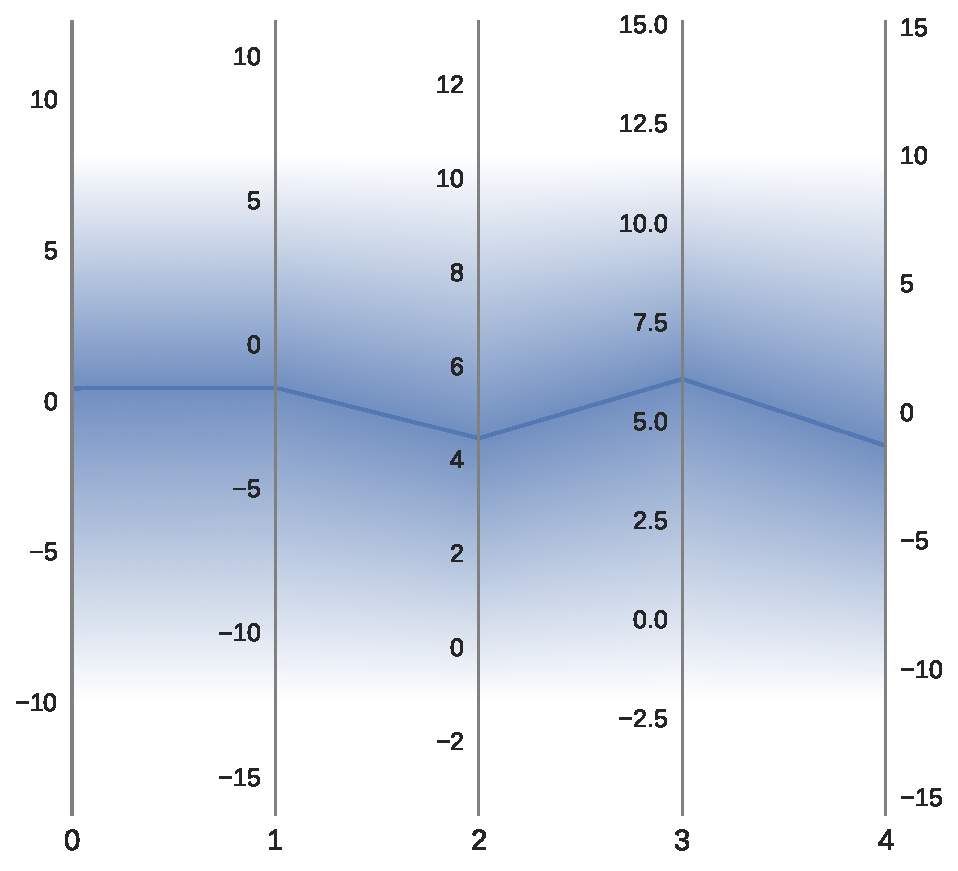
\includegraphics[width=4.5cm]{h_clustering_1.pdf} \hfill
        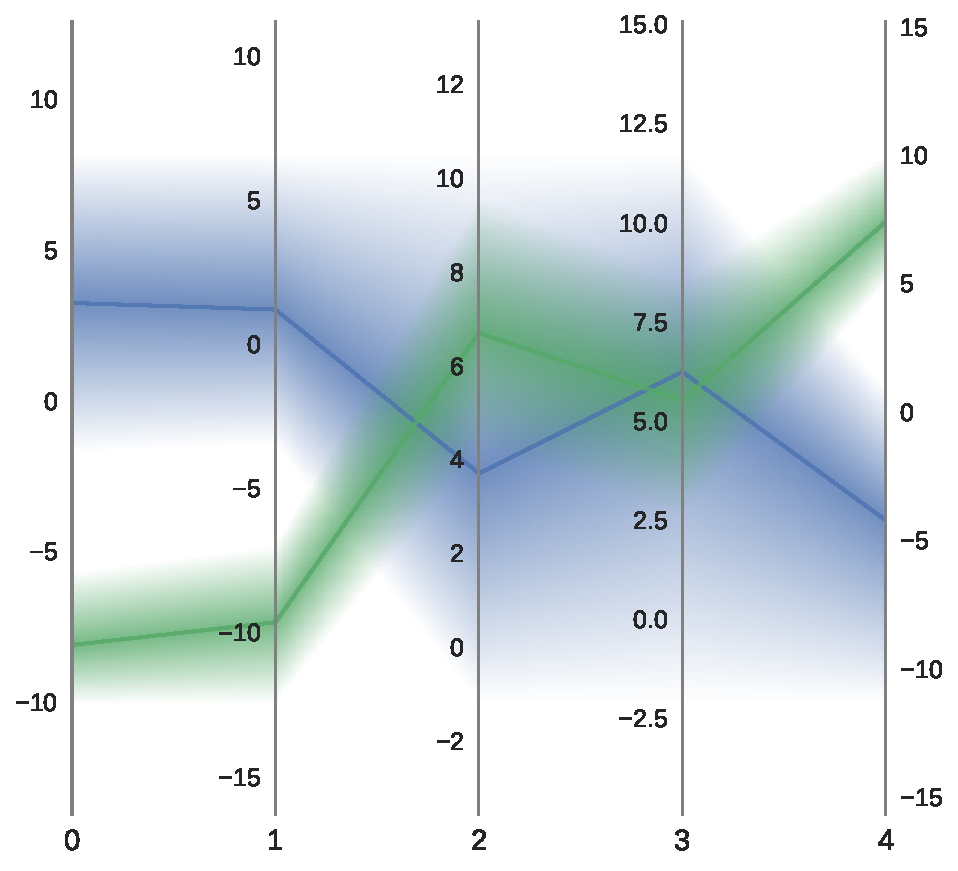
\includegraphics[width=4.5cm]{h_clustering_2.pdf} \hfill
        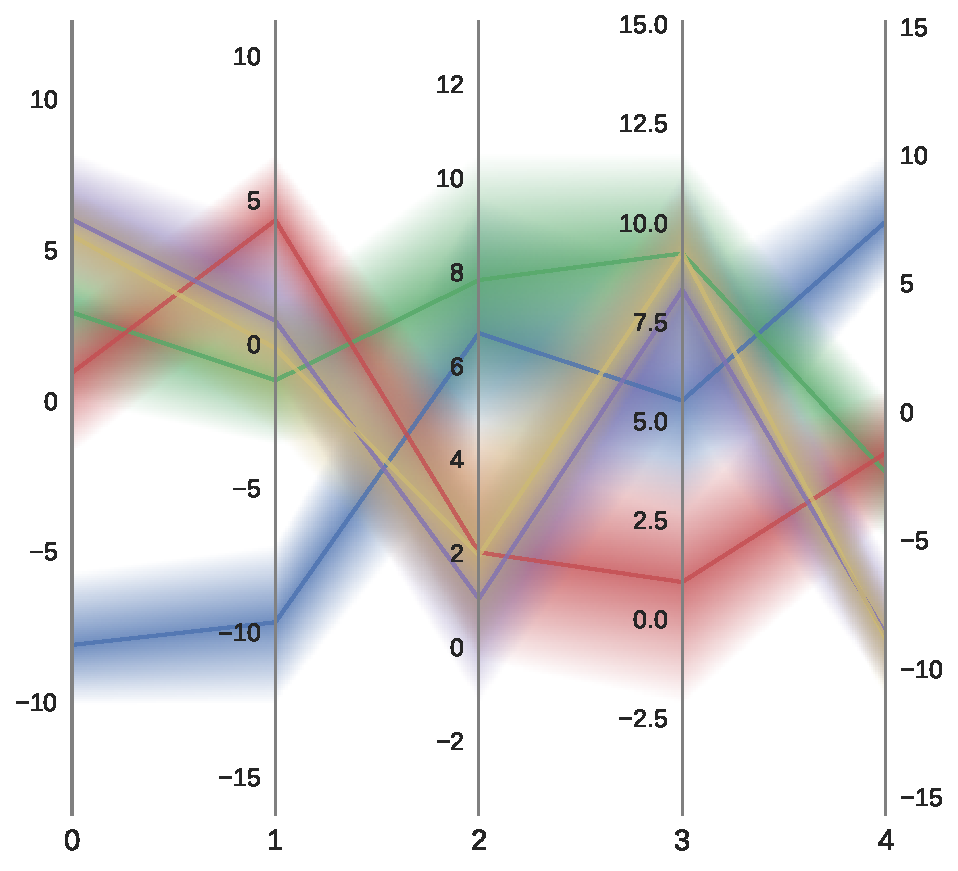
\includegraphics[width=4.5cm]{h_clustering_5.pdf} \hfill
    \caption{Иерархические графики начиная с корня и заканчивая большим количеством кластеров}
    \label{hierarchical_coords}
\end{figure}


Иерархические графики в параллельных осях представляют собой метод визуализации не объектов, а иерархических
кластерных структур --- дендрограмм. Вместо визуализации конкретных объектов будем
визуализировать сообщества похожих объектов. Чтобы визуализировать сообщества (кластеры)
нужно выбрать некоторые статистики, например среднее, стандартное отклонение, максимум, минимум. Среднее нарисуем обычной линией, а 
стандартное отклонение отобразим полупрозрачным градиентом (Рис.\ref{hierarchical_coords}).
Так график становится более читабельным, а детализация регулируется с
помощью включения новых кластеров из дендрограммы.\cite{hierarchical}

\begin{figure}[htb]
    \centering
    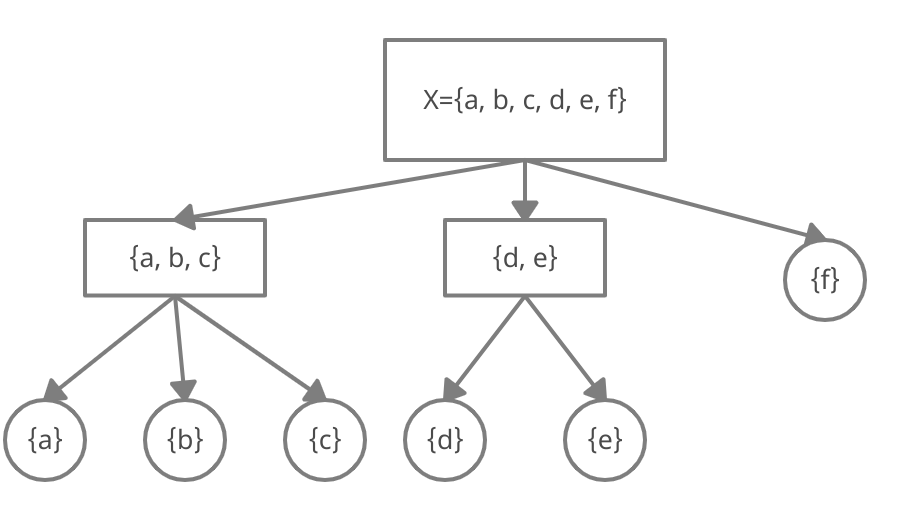
\includegraphics[width=9cm]{hierarchical_graph.png}
    \caption{Дендрограмма}
    \label{hierarchical_partition}
\end{figure}


\noindent \large \textbf{Формализуем определение.}

\vspace{10pt}

\noindent Пусть $X=(x_1,\ldots,x_n)$ -- выборка, где $x_i\in \mathbb{R}^n$. 

\noindent Назовем множество $P$ m-разбиением множества X на m-подмножеств $\{P_1,\ldots,P_m\}$
такое, что:
\begin{align}
    \notag &1. P_i \cap  P_j = \oslash, \hspace{10px} \forall i,j =\overline{1,m} \\
    \notag &2. \bigcup\limits_{i=1}^{m} P_i = X 
\end{align}

\noindent Организуем иерархическую структуру (дендрограмму) в виде дерева, где корню соответствует $X$, 
а каждая вершина сопоставлена элементу разбиения родительской вершины (Рис.\ref{hierarchical_partition})
После построения дендрограммы необходимо выбрать выбрать какие разбиения будем отображать. 
Часто в качестве критерия отбора используется глубина дерева.

\section{Проблемы построения}

\subsection{Основные проблемы}
Как и любые средства визуализации график в параллельных осях обладает достоинствами и недостатками.

К достоинствами можно отнести то, что мы можем визуализировать пространства практически
любой размерности. Также график обладает высокой вариативностью и простой интерпретацией, но за
вариативность мы платим большим количеством гиперпараметров, которые нужно подбирать. 
Главный недостаток -- потеря читаемости на больших и ''грязных'' выборках. 
Некоторые модификации графика частично решают эту проблему, но так мы можем потерять важную информацию о конкретных объектах.
Помимо прочего у исследователя могут возникать естественные вопросы при построении:

\begin{itemize}
    \item В каком порядке расположить оси?
    \item В какую сторону направлять оси?
    \item Как много объектов отобразить?
    \item Какой масштаб выбрать для каждой оси?
\end{itemize}

\noindent Обычно ответы на них ложатся на плечи самого исследователя и не всегда подбор этих гиперпараметров эффективен и объективен.
Далее мы введем формальные критерии качества для ответов на первые два вопроса.

\subsection{Выбор порядка и направления осей}
Чтобы формализовать ''правильный'' порядок и направление осей необходимо понять, когда и почему
человек лучше воспринимает зависимости на графике. Выделим основные причины:

\begin{itemize}
    \item Линии редко пересекаются между собой.
    \item Монотонная зависимость между двумя соседними координатами.
    \item Направление осей вверх (от меньшего к большему).
    \item Слишком ''шумные'' зависимости где-нибудь на последних (справа) осях\footnote{Человеку привычнее воспринимать 
    информацию слева направо.}
\end{itemize}

\begin{figure}[htb]
    \centering
       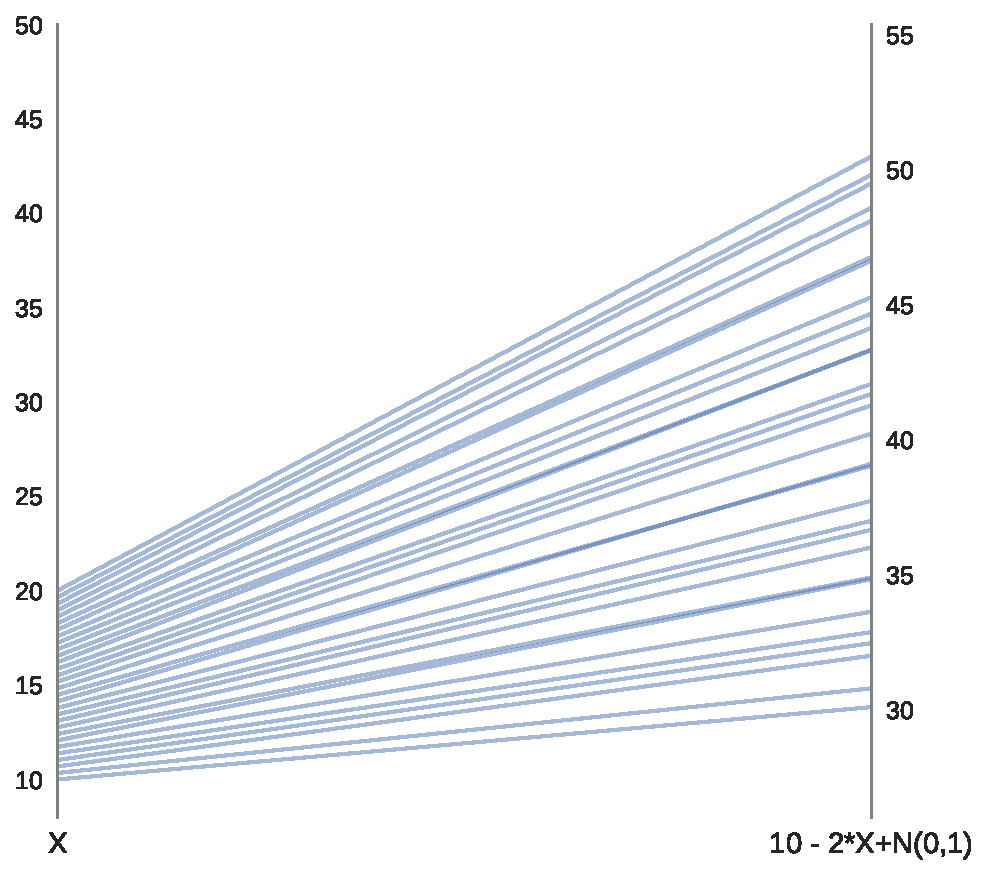
\includegraphics[width=5cm]{monotone_good_example.pdf} \hfill
       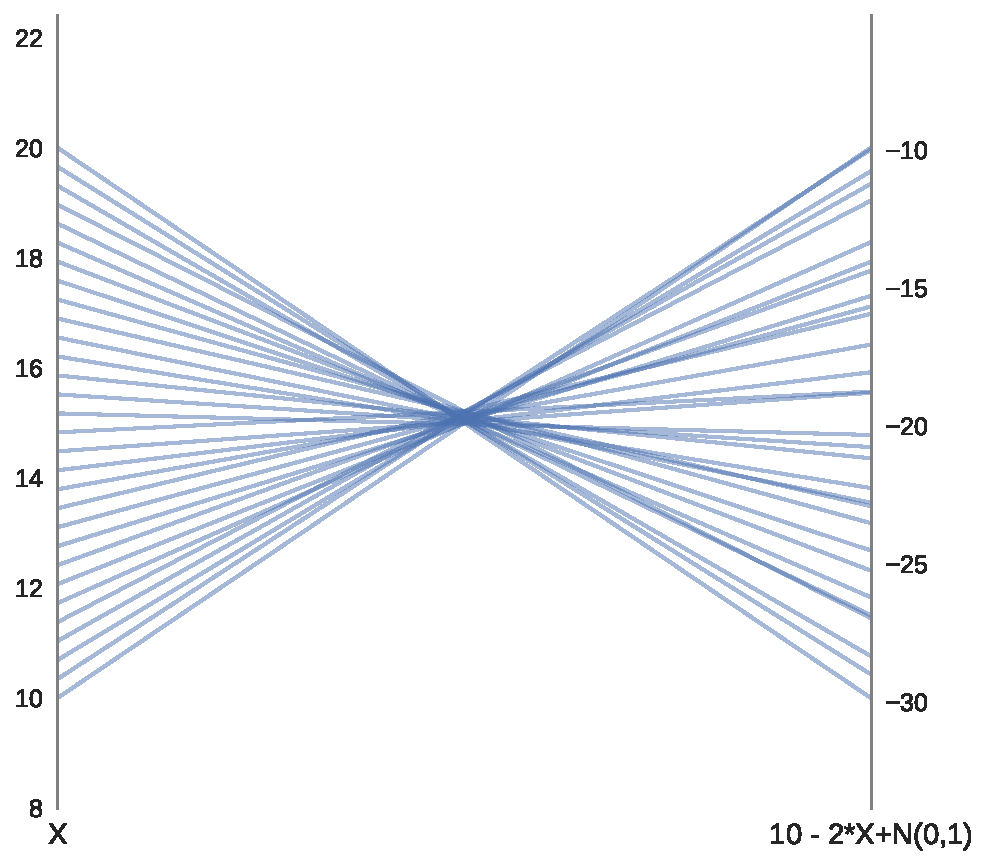
\includegraphics[width=5cm]{monotone_bad_example.pdf} \hfill
       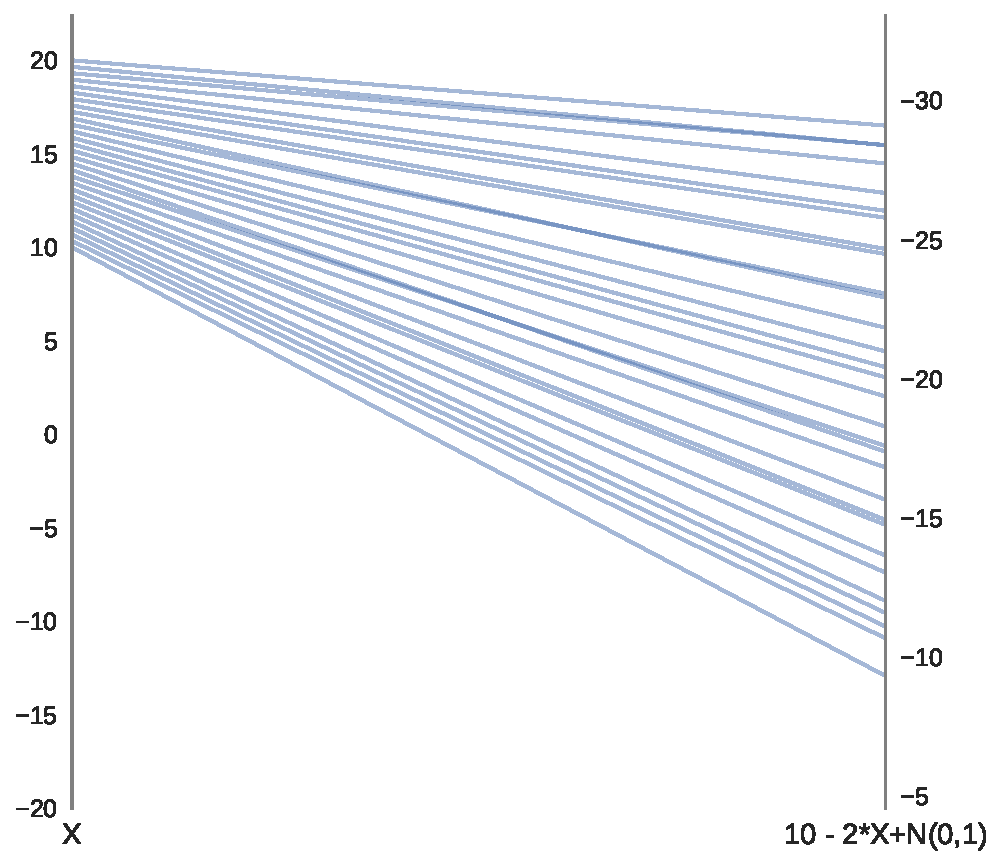
\includegraphics[width=5cm]{monotone_bad_with_direction.pdf} \hfill
   \caption{Xорошо читаемая зависимость. Плохо читаемая зависимость. Предыдущий пример с перевернутой осью}
   \label{monomote_example}
\end{figure}

Приведем некоторые примеры плохого и хорошего поведения графика. На Рис. \ref{monomote_example} в первом случае мы видим хорошо читаемую зависимость между осями -- она монотонна и возрастает.
Во втором случае зависимость тоже монотонна, но убывающая. Из-за этого мы получаем большое 
количество пересечение линий, что сильно сказывается на читаемости т.к. сложнее проследить за каждой отдельной линией. В случае более ''шумных'' зависимостей ситуация может усугубляться еще сильнее.
Третий случай дублирует второй, но вторая ось направлена в другую сторону, что позволяет увидеть монотонную зависимость.


\subsubsection*{Корреляция}
Для введения метрики качества нам понадобится величина, характеризующая меру монотонной зависимости
между объектами.

\newpage

\noindent \textit{Пусть даны две выборки $X=(x_1, \ldots ,x_n), Y=(y_1,\ldots ,y_n)$.}

\noindent \textit{Корреляция Пирсона вычисляется по следующей формуле:}
$$
    \rho_{XY} = 
    \frac{\sum\limits_{i=1}^{n}(x_i-\overline x)(y_i-\overline y)}
    {\sqrt{\sum\limits_{i=1}^{n}(x_i-\overline x)^2\sum\limits_{i=1}^{n}(y_i-\overline y)^2}}, 
    \hspace{15px} \left\lvert \rho_{XY} \right\rvert \leq 1
$$   
\textit{где $\overline x, \overline y$ -- выборочные средние.}

\vspace{10pt}

\noindent Заметим, что корреляция Пирсона не всегда хорошо проявляет при поиске монотонной зависимости между
выборками.\footnote{Корреляцию Пирсона также можно использовать в дальнейших выкладках.}
Введем меру, лишенную этого недостатка:

\vspace{10pt}

\noindent \textit{Корреляция Спирмена вычисляется по следующей формуле:}

$$
    r_{XY} = 
    \frac{\sum\limits_{i=1}^{n}(R_i-\overline R)(S_i-\overline S)}
    {\sqrt{\sum\limits_{i=1}^{n}(R_i-\overline R)^2\sum\limits_{i=1}^{n}(S_i-\overline S)^2}},
    \hspace{15px} \left\lvert r_{XY} \right\rvert \leq 1
$$
\noindent \textit{где $R_i$ -- ранг наблюдения $x_i$, $S_i$ -- ранг наблюдения $y_i$}

\subsubsection*{Функционал качества}
Наконец, мы готовы ввести функционал, характеризующий степень качества размещения осей.

\vspace{10pt}

\noindent \textit{Пусть $\pi = (\pi_1, \ldots , \pi_n)$ перестановка множества $\{1,\ldots, n\}$, где $n$ размерность пространства.}

\noindent \textit{Мы хотим максимизировать такой функционал:}
$$\mathcal{R} (X,\pi)=\sum\limits_{i=1}^{n-1}|r_{X^{\pi_i}X^{\pi_{i+1}}}| \rightarrow \max\limits_\pi$$
\textit{где $r_{X^iX^j}$ -- Корреляция Спирмена между  $i$ координатой и $j$ координатой.}

\vspace{10pt}
Заметим, что функционал может поощрять монотонно убывающие зависимости, что, вообще говоря, приведет к
большому количеству пересечений линий между осями. Но нетрудно показать, что после нахождения порядка линий можно выбрать направления осей так, 
чтобы пересечения между линиями были минимальны.

Смысл данной формулы состоит в том, что мы хотим найти расположение осей максимизирующие
сумму корреляций между соседними парами осей на графике. Так мы можем найти максимально ''полезные'' 
зависимости между признаками.


\subsubsection*{Оптимизация функционала качества}

\begin{figure}[htb]
    \centering
       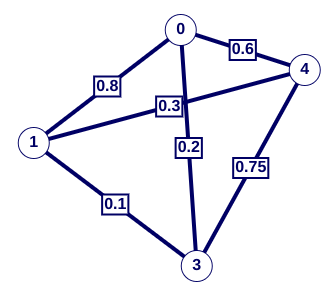
\includegraphics[width=7cm]{graph_example_1.png} \hfill
       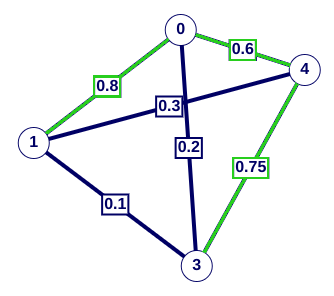
\includegraphics[width=7cm]{graph_example_2.png} \hfill
   \caption{Вершины соответствуют координатам, а ребра попарным корреляциям}
   \label{graph_example}
\end{figure}


Максимизация этого функционала тесно связна с задачей ''о самом длинном пути'' в теории графов.

\vspace{5pt}

\noindent \textbf{Задача о самом длинном пути} --   это задача поиска простого пути максимальной длины в заданном графе.
 Является NP-трудной и не может быть решена за 
 полиномиальное время для произвольных графов. Покажем связь нашей задачей:

 \vspace{10pt}

 \noindent \textit{Пусть $X=(x_1,\ldots,x_n)$ -- выборка, где $x_i\in \mathbb{R}^n$.}

 \vspace{5pt}

 \noindent \textit{Построим связный граф $G(V,E)$, где каждая вершина $u^i \in V$ соответствует
 i-ой координатe (i-ой оси на графике), а каждому ребру $\{u^i,u^j\} \in E$ сопоставим вес равный $|r_{X^iX^j}|$. (Рис. \ref{graph_example})}

\vspace{10pt}

Если в таком графе мы найдем самый длинный простой путь, то задача максимизации функционала будет решена. 
Простейший перебор имеет асимптотику $O(n!)$, но помощью методов динамического программирования можно ее можно улучшить. Заметим, что 
график в параллельных осях стоит использовать при $n < 15$, иначе график перестанет быть читаемым.

\section{Пример использования}
Для примера был выбран датасет ''The Boston Housing Dataset''. Предварительно убраны категориальные признаки, 
а также проведена кластеризация методом K-means для большей наглядности.

\begin{figure}[htb]
    \centering
    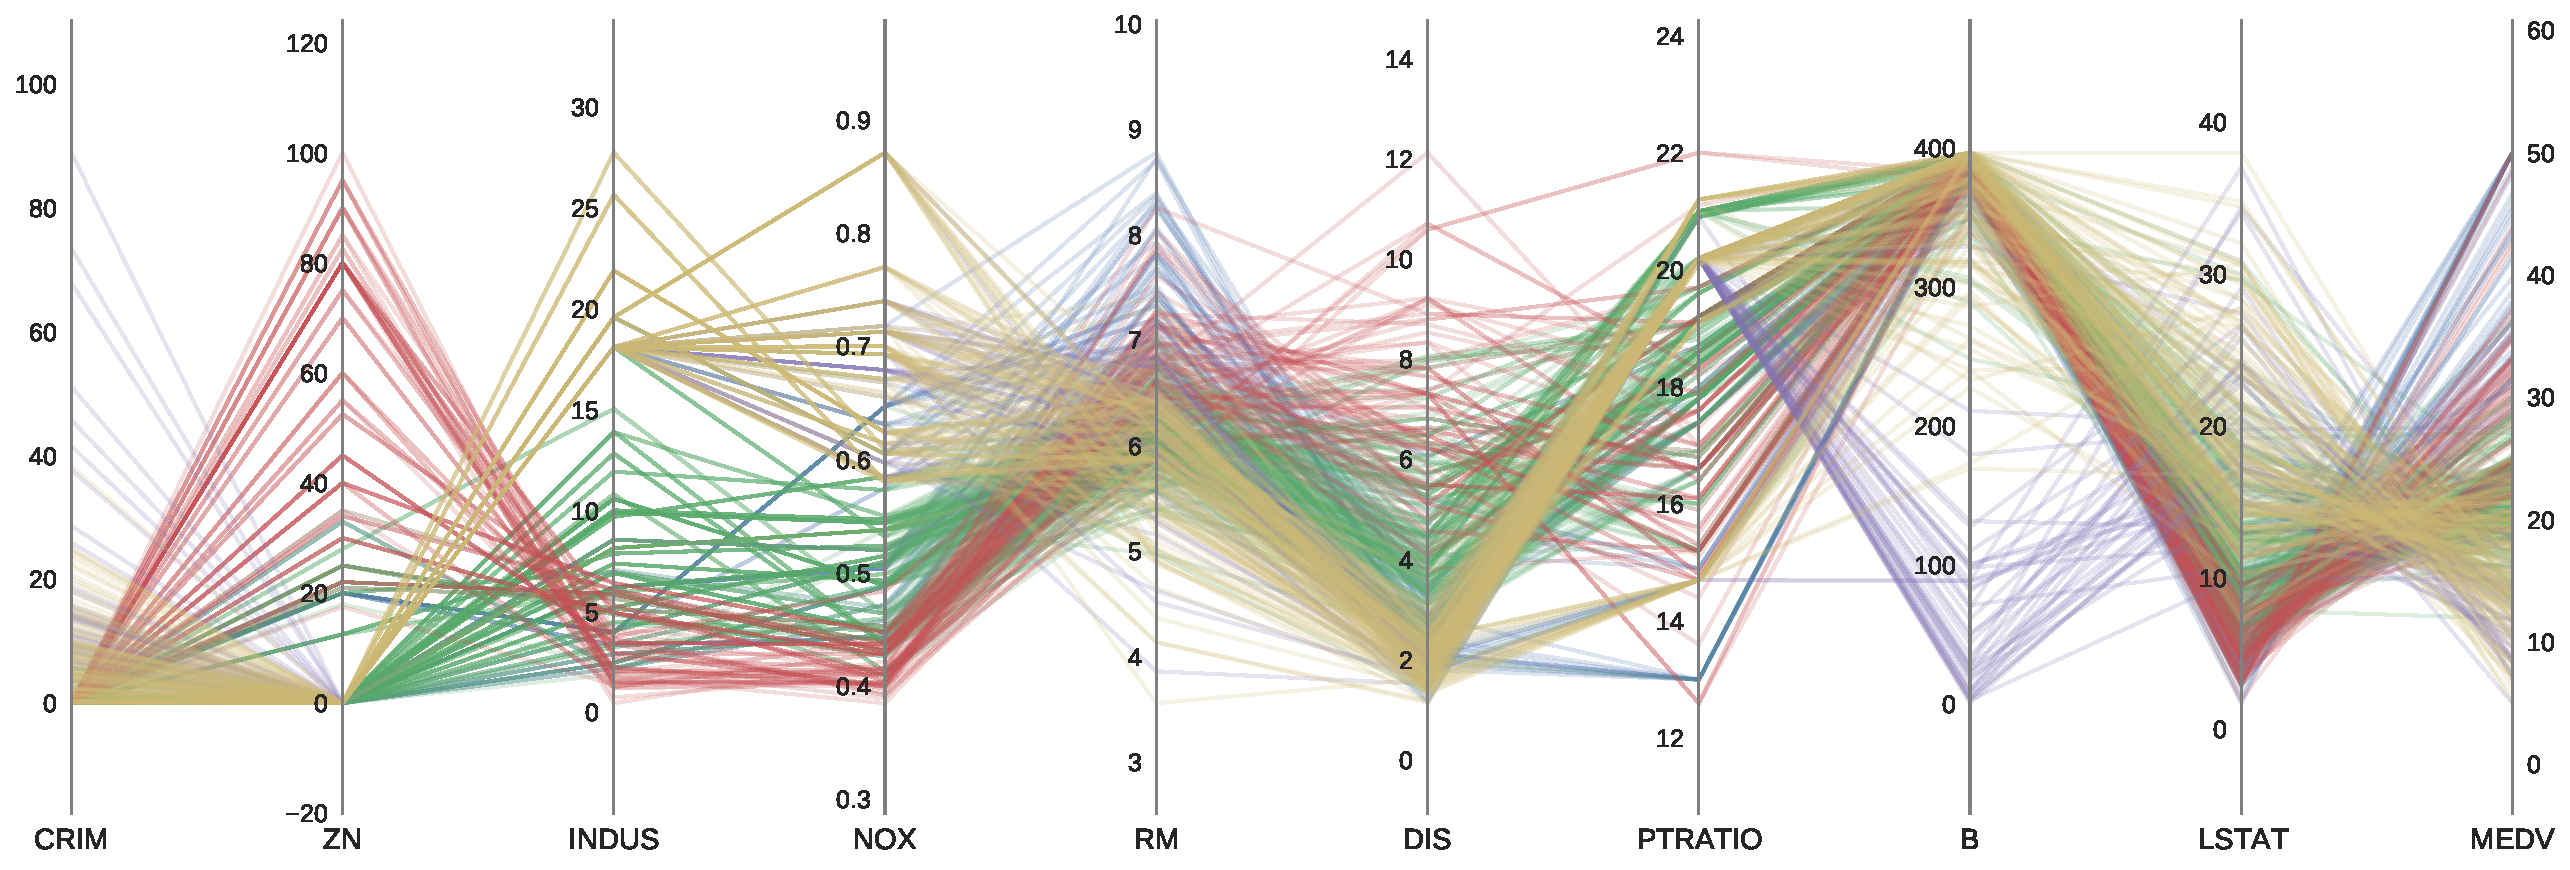
\includegraphics[width=15cm]{housing_example_1.pdf}\\
    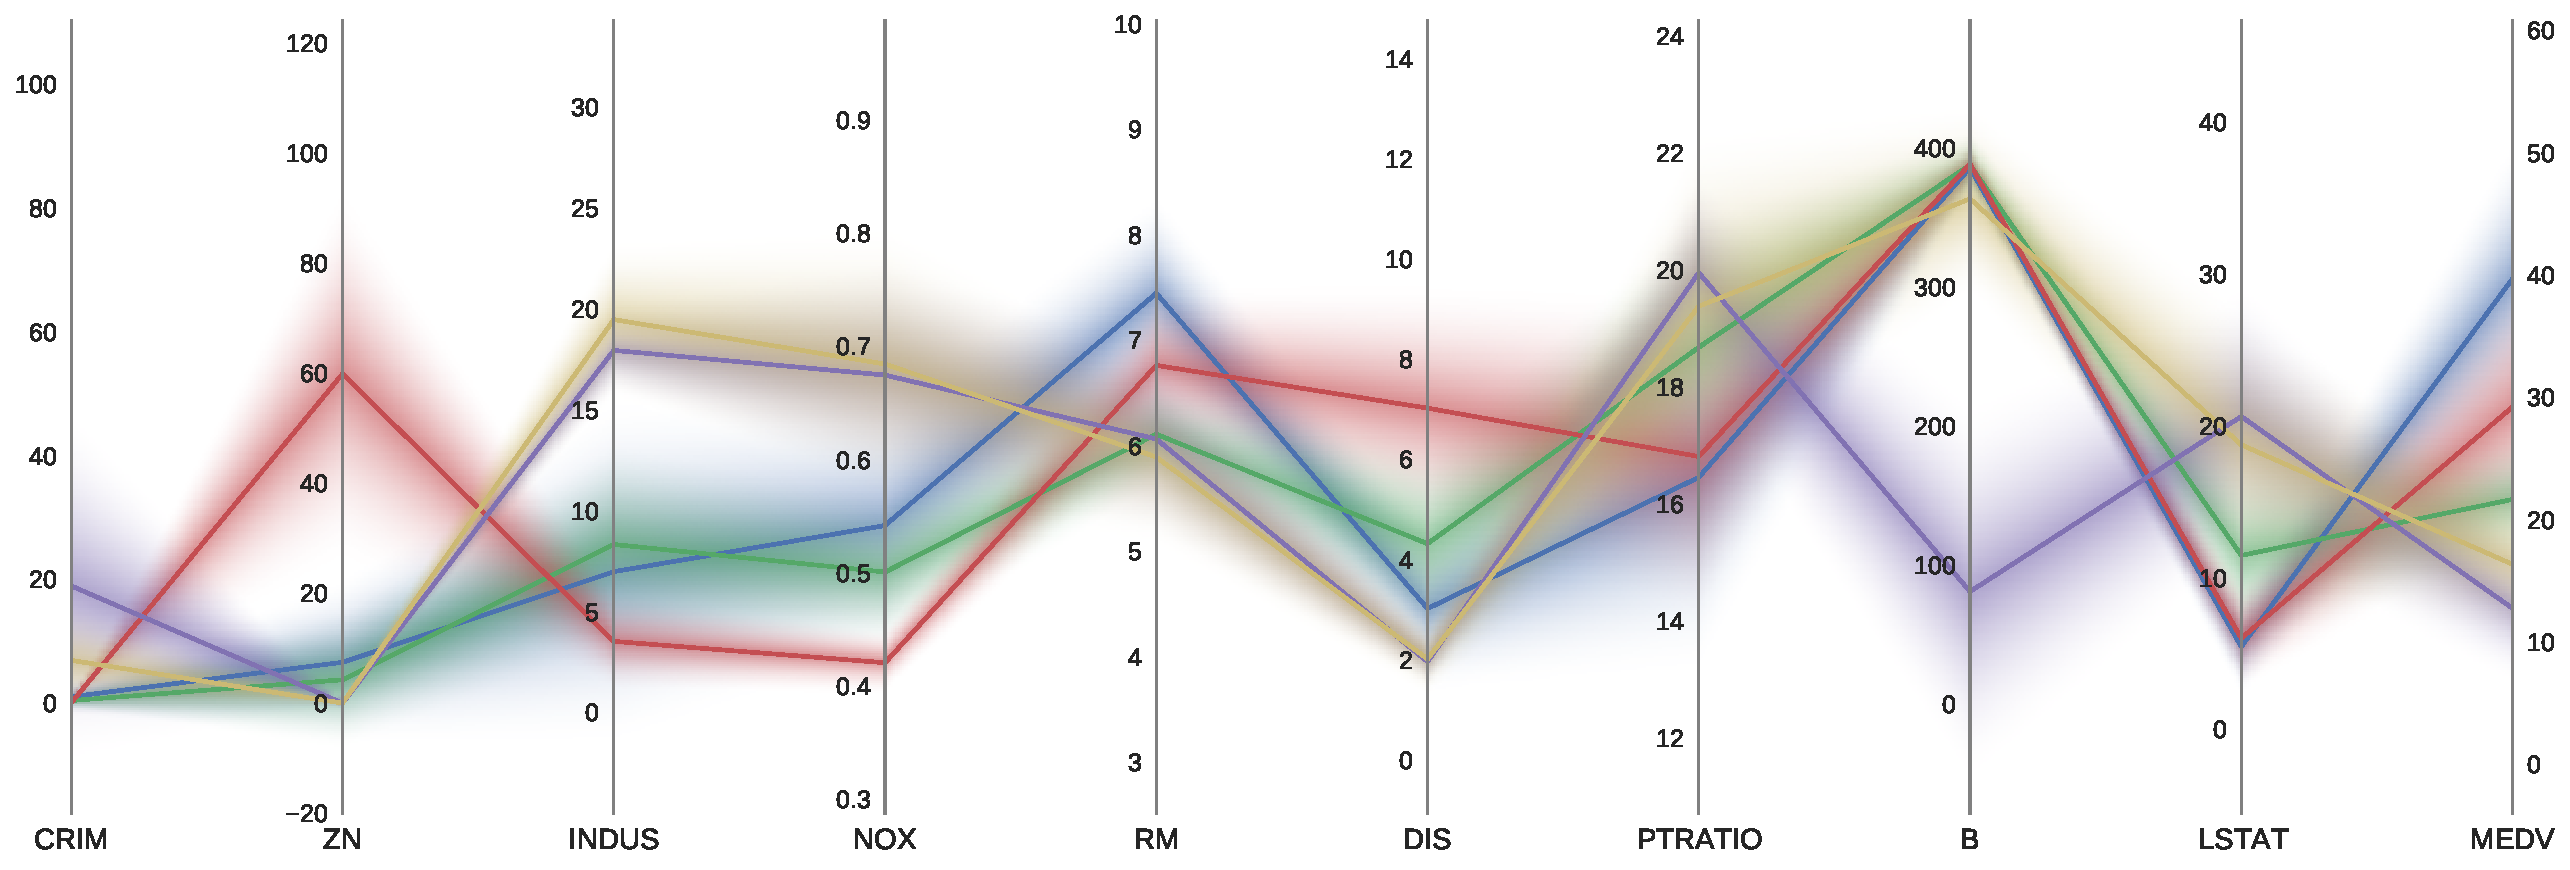
\includegraphics[width=15cm]{housing_example_3.pdf}
    \caption{Графики в параллельных осях без выбора порядка}
    \label{house_example_1}
\end{figure}

На Рис.\ref{house_example_1} представлены графики без выбора порядка признаков. График получается
довольно ''шумным'' -- много пересечений линий, сложно заметить зависимости между признаками.


\begin{figure}[htb]
    \centering
    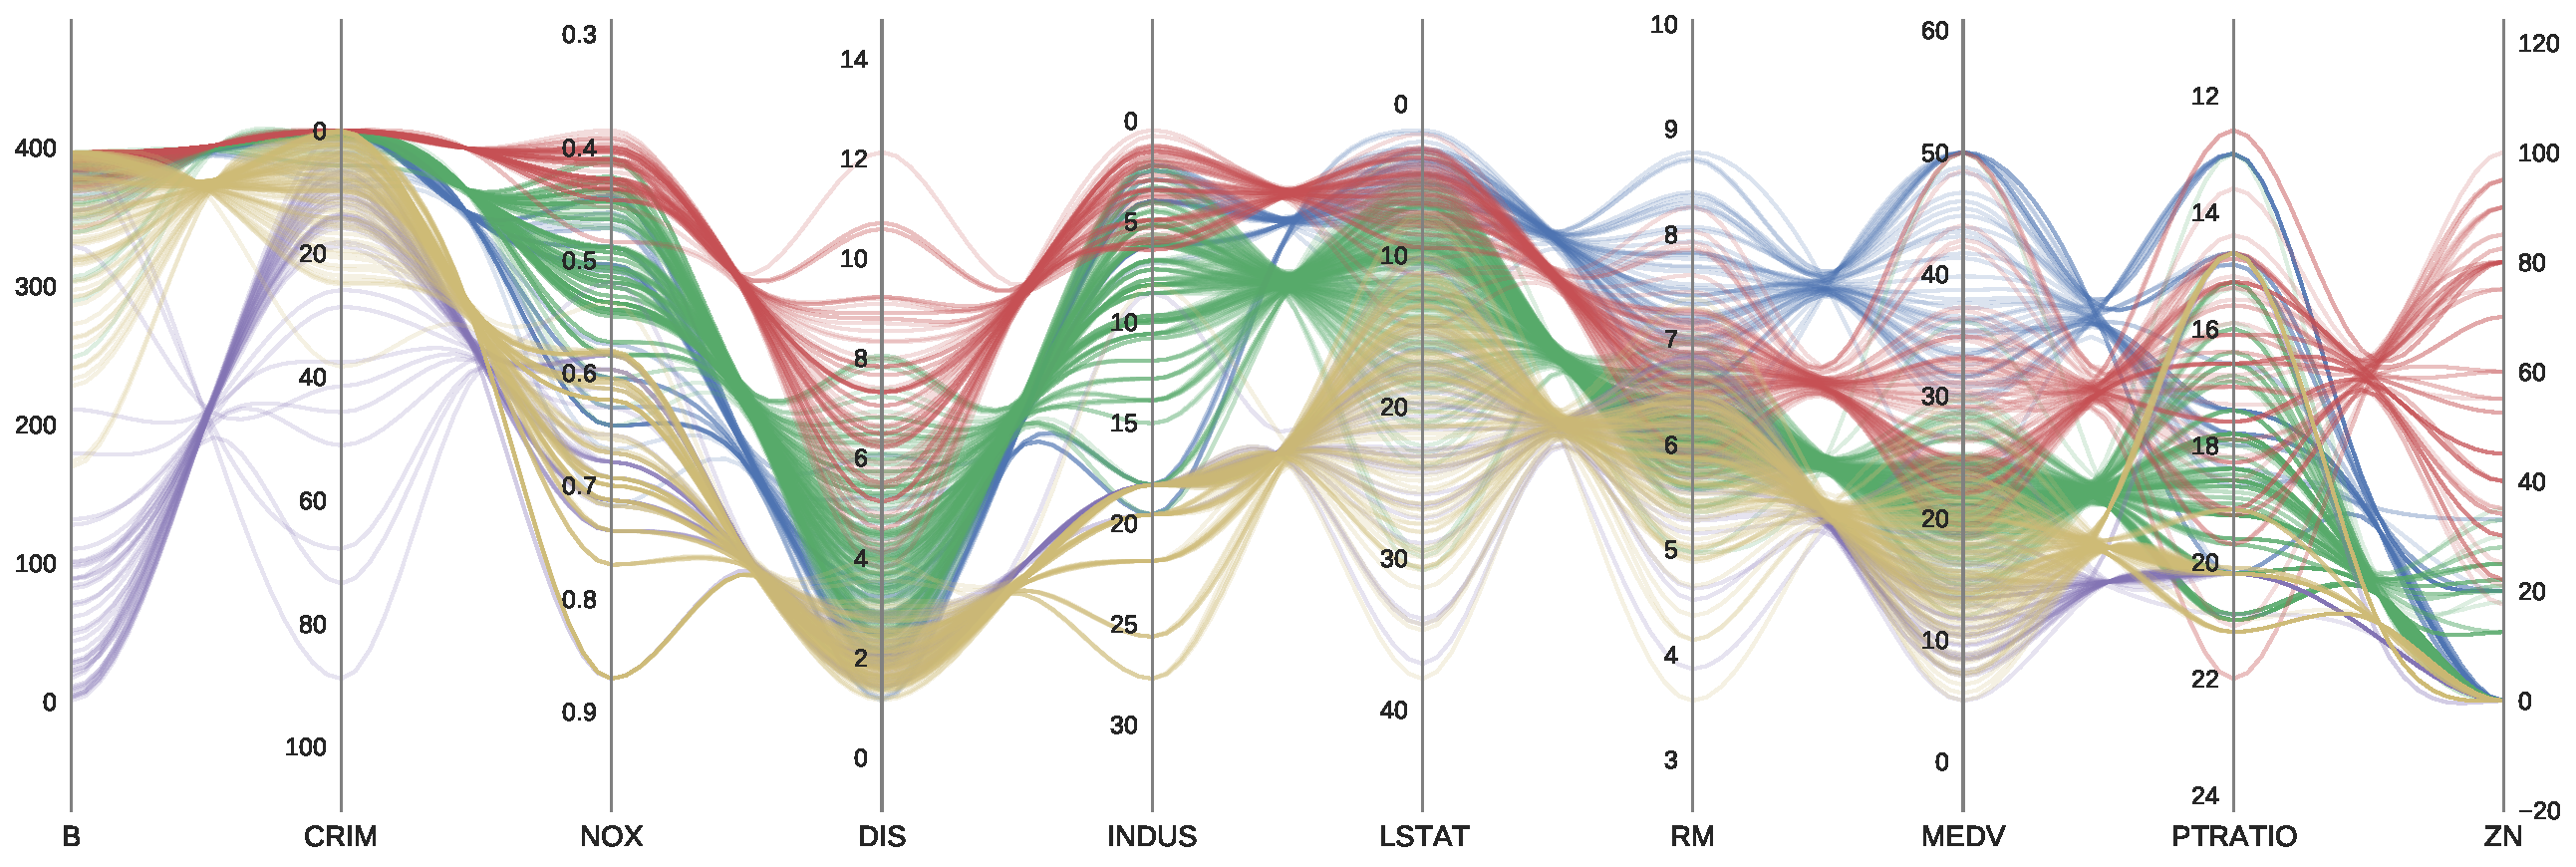
\includegraphics[width=15cm]{housing_example_4.pdf}\\
    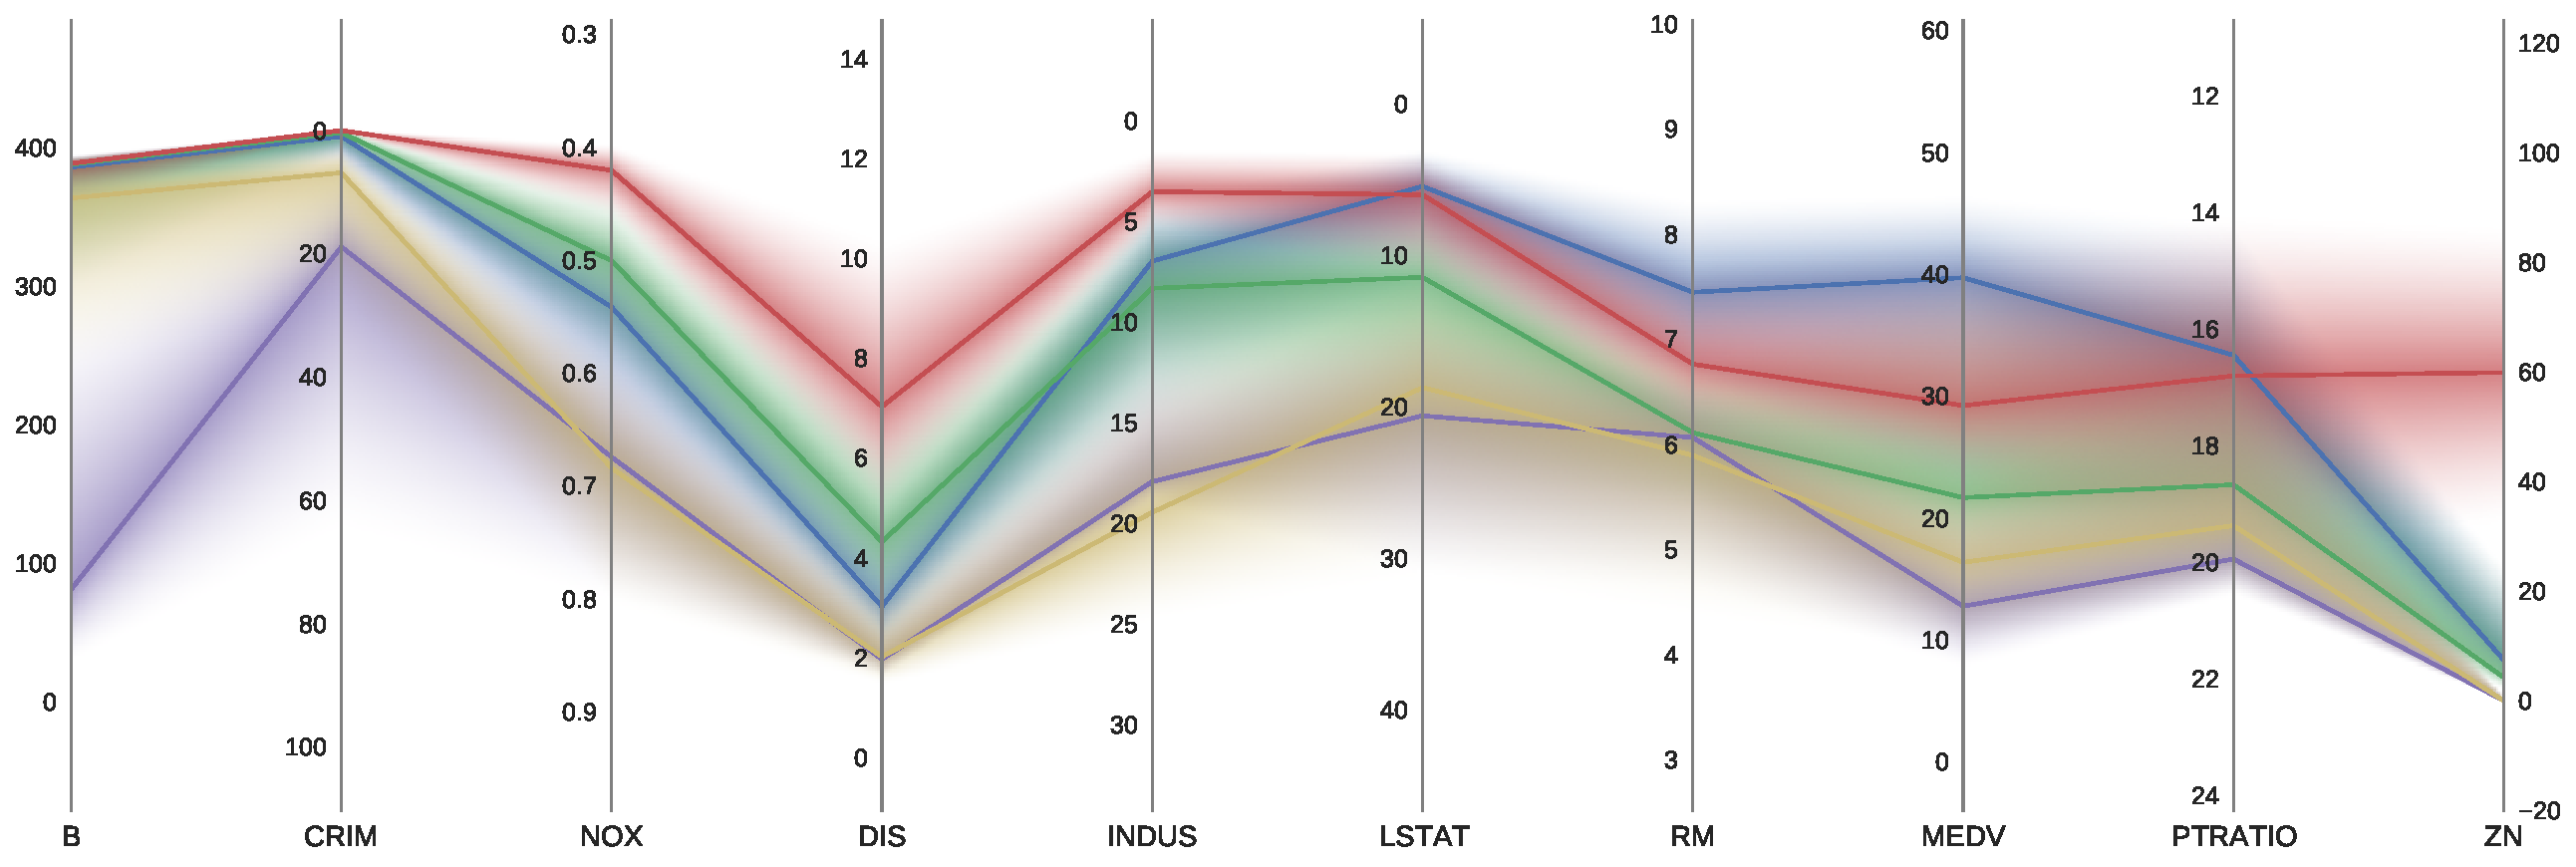
\includegraphics[width=15cm]{housing_example_5.pdf}
    \caption{Графики в параллельных осях с выбором порядка}
    \label{house_example_2}
\end{figure}

На Рис. \ref{house_example_2} проиллюстрированы графики после нахождения оптимального порядка осей.
После оптимизации нам проще разглядеть структуру кластеров не только в совокупности, но и между кластерами. 
Для примера рассмотрим ось NOX(количество азота в воздухе) и DIS(сумма расстояний от центров занятости). До оптимизации
мы не могли наблюдать монотонно убывающую зависимость (чем больше NOX, тем меньше DIS), но после она четко видна.
Таким образом нахождение оптимального порядка с точки зрения введенного функционала максимизирует 
число интерпретируемых зависимостей между осями. Но нужно заметить, что нам не гарантируется, что мы обнаружим все ''хорошие'' зависимости так как
каждый признак может ''взаимодействовать'' максимум с двумя другими признаками на графике.


\section{Библиотека визуализации}
\subsection{Обзор текущих прикладных средств}
Несмотря на то, что написано большое количество работ о графиках в параллельных осях, 
существует лишь несколько программ, общедоступных для работы с ними.
Например: ELKI, GGobi, Mondrian, Orange и ROOT. Отдельно выделяется D3.Parcoords.js -- 
мощная библиотека на языке JavaScript, посвященная только графикам в параллельных осях.
В python в библиотеке pandas есть лишь его базовая версия. В других же популярных
python библиотеках нет даже этого.

Удивительно, что такое мощное средство визуализации обходят стороной разработчики библиотек. 
Возникает желание создать собственный продукт со всеми возможными подходами к рисованию графика 
в параллельных осях.
\subsection{Цели и задачи библиотеки}
В первую очередь необходимо заметить, что библиотека пишется на базе 
matplotlib. Это мощная низкоуровневая библиотека, умеющая рисовать всевозможные 
статические диаграммы. Статичность диаграммы можно считать как недостатком, так и достоинством\footnote{
В сфере визуализации монополия на использование интерактивных графиков отдана JavaScript и
его библиотекам. Статичные графики обычно рисуют с помощью matplotilb или библиотек, созданных на его базе.}. 
С одной стороны интерактивность в случае графиков в параллельных осях существенно ускоряет построение
эстетичного графика, но с другой это может излишне перегружать и усложнять взаимодействие
пользователя с библиотекой, а также существенно уменьшить спектр возможностей. Библиотека на базе 
matplotilb позволит пользователю не только тончайшим образом настраивать вид графика, но и быстро
получить красивый и информативный график ''из коробки''.
\footnote{Примером может служить библиотека seaborn, написанная на базе matplotlib, но
использующая высокоуровневые функции, позволяющие избегать утомляющей настройки.}


\subsection{Технические особенности}
\begin{itemize}
    \item Простой высокоуровневый интерфейс. Как и в библиотеке seaborn методы могут принимать pandas.DataFrame,
    обычные numpy массивы или списки -- для всего единый интерфейс.\footnote{Пока что в качестве 
    входных данных доступен только pandas.DataFrame}
    \item Возможность сохранения графика в любой формат, поддерживаемый matplotlib
    \item Нативно встраивается в любые программные оболочки, поддерживающие matplotlib.
    \item Возможность кастомизации уже готового графика.
\end{itemize}


\subsection{Возможности библиотеки}
\begin{itemize}
    \item Построение классических графиков в параллельных осях
    \begin{itemize}

        \item Возможность рисовать гладкие линии.
        \item Возможность ''связывания'' линий кластеров.
    \end{itemize}
    \item Построение иерархических графиков
    \begin{itemize}
        \item Отрисовка полупрозрачного градиента.
        \item Работа с иерархическими кластерами(дендрограммами).
    \end{itemize}
    \item Дополнительно \textit{(пока не реализовано)}
    \begin{itemize}
        \item выделение подмножества линий в  диапазоне значений одной из осей.
        \item нахождение оптимального расположения осей.
        \item создание иерархических кластеров на основе входящей выборки.
    \end{itemize}
\end{itemize}

\section{Заключение}
В работе были рассмотрены основные виды графиков в параллельных осях, их достоинства и недостатки, 
предложен метод повышения читаемости и информативности за счет выбора порядка и направления. Эксперименты
показали, что дискретная оптимизация введенного функционала качества улучшает восприятие графика и позволяет найти 
нетривиальные зависимости в данных. Удалось связать оптимизацию данного функционала с NP-полной задачей 
\textit{''О максимальном пути''} в полном графе с неотрицательными ребрами. Улучшение асимптотики
решения данной задачи открытая проблема. Вообще говоря, данный функционал не единственный вариант оптимизации порядка осей и это требует
дальнейших исследований. Также была разработана \href{https://github.com/Tytskiy/hpcoords}{open-source библиотека} на языке Python для построения данных графиков.

\newpage

\begin{thebibliography}{99}
    \bibitem{inselberg_1985} Inselberg A., Dimsdale B. Parallel coordinates: 
    a tool for visualizing multi-dimensional geometry 
    //Proceedings of the First IEEE Conference on Visualization: 
    Visualization90. – IEEE, 1990. – С. 361-378.
    \bibitem{state_of_the_art} Heinrich J., Weiskopf D. State of the Art of Parallel Coordinates 
    //Eurographics (STARs). – 2013. – С. 95-116.
    \bibitem{bundling} Heinrich J. et al. Evaluation of a bundling technique for parallel coordinates 
    //arXiv preprint arXiv:1109.6073. – 2011.
    \bibitem{hierarchical} Fua Y. H., Ward M. O., Rundensteiner E. A. Hierarchical parallel coordinates
     for exploration of large datasets. – IEEE, 1999. – С. 43-508.
     \bibitem{data_analysis} Wegman E. J. Hyperdimensional data analysis using parallel coordinates 
     //Journal of the American Statistical Association. – 1990. – Т. 85. – №. 411. – С. 664-675. 
     \bibitem{inselberg_2009} Inselberg A. (2009) Parallel Coordinates. In: LIU L., ÖZSU M.T. (eds)
      Encyclopedia of Database Systems. Springer, Boston, MA
\end{thebibliography}
\end{document}